\documentclass[10pt,letterpaper]{article}

% ---------------------------------------------------------------------------
% The Stubborn Prior -- research proposal (arXiv-style)
% Build: latexmk -pdf main.tex   (see README.md)
% ---------------------------------------------------------------------------

\usepackage[T1]{fontenc}
\usepackage[utf8]{inputenc}
\usepackage{mathptmx}
\usepackage[scaled=0.92]{helvet}
\usepackage[margin=1in]{geometry}
\usepackage{microtype}
\usepackage{amsmath,amssymb,amsthm}
\usepackage{booktabs}
\usepackage{array}
\usepackage{graphicx}
\usepackage{caption}
\usepackage{enumitem}
\usepackage{xcolor}
\usepackage{tikz}
\usetikzlibrary{arrows.meta,positioning,calc,shapes.geometric}
\usepackage{pgfplots}
\pgfplotsset{compat=1.18}
\usepackage[round,authoryear]{natbib}
\usepackage[colorlinks=true,linkcolor=black,citecolor=black,urlcolor=black]{hyperref}

\captionsetup{font=small,labelfont=bf}
\setlist{nosep,leftmargin=*}
\setlength{\parskip}{0.25em}

% Visible placeholders for values that must be recovered from the run logs.
\definecolor{todored}{rgb}{0.65,0.05,0.05}
\newcommand{\todo}[1]{\textcolor{todored}{\textbf{[TODO: #1]}}}

\newcommand{\Hset}{\mathcal{H}}
\newcommand{\Aset}{\mathcal{A}}
\newcommand{\Yset}{\mathcal{Y}}
\newcommand{\STOP}{\mathrm{STOP}}
\newcommand{\CONT}{\mathrm{CONTINUE}}
\newcommand{\rep}{\mathrm{rep}}
\newcommand{\Bayes}{\mathrm{Bayes}}
\newcommand{\rev}{\mathrm{rev}}
\newcommand{\E}{\mathbb{E}}
\newcommand{\Ind}{\mathbb{1}}
\newcommand{\Ustop}{U_{\mathrm{stop}}}
\newcommand{\Lstop}{L_{\mathrm{stop}}}
\newcommand{\Bop}{\mathcal{B}}
\DeclareMathOperator*{\argmax}{arg\,max}

\title{\Large\bfseries The Stubborn Prior:\\ When False Scientific Beliefs Distort AI Research Policy}
\author{\todo{author list and affiliations}}
\date{Research proposal, \today}

\begin{document}
\maketitle

\begin{abstract}
\noindent
If an AI scientist starts with a plausible but wrong theory, does it become confirmation biased? The obvious test is to compare an agent given a false prior with an agent given a neutral one. That test is confounded: a rational scientist with a false prior should already choose different experiments and end with different beliefs. So we ask a narrower question. Given the belief state the model itself reports, does it do science the way a rational scientist with that same belief state would?

We build finite scientific worlds in which every hypothesis, experiment, outcome likelihood, and cost is known, which lets us run an exact Bayesian scientist initialized with the model's own prior. In four preliminary study families, once we normalized for prior differences correctly, we found little evidence that false-prior models refuse contradictory evidence. That pushed us to a different hypothesis: false priors may leave local reasoning mostly intact while distorting the decisions that control whether contradictory evidence is ever collected. Our two primary studies test whether models avoid a belief-threatening experiment their own prior says to run, and whether they stop investigating when their own prior says to continue. A well-powered null is a real result here: it would mean naive false-prior comparisons can overstate the problem.
\end{abstract}

% ===========================================================================
\section{Introduction}
\label{sec:intro}

The original question was simple. If an AI scientist starts with the wrong scientific belief, does it become confirmation biased?

It turns out that question does not quite work.

Take two scientists. One thinks theory $H'$ is 80\% likely, the other thinks it is 20\% likely. Even if both are perfectly rational, they should choose different experiments, value information differently, stop at different times, and finish with different posteriors. Bayes itself predicts a difference. So when a false-prior model behaves differently from a neutral model, that is not evidence of bias. It is what a correct scientist would also do. In one line,
\begin{equation*}
\text{false prior} \;\not\Rightarrow\; \text{irrationality}.
\end{equation*}

The distinction we need is
\begin{equation*}
\text{belief error} \;\neq\; \text{reasoning error} \;\neq\; \text{research-policy error}.
\end{equation*}
A scientist can be wrong without being irrational. A scientist can also reason correctly about each observation and still run bad science, because the theory it holds decides which observations get made. As models move from answering questions to deciding what to test, whether an anomaly is worth chasing, and when a question is done, the second kind of failure is the one that matters.

\paragraph{The sharper question.}
Instead of comparing the false-prior model to a neutral model, we compare it to a rational scientist who believes exactly what the model says it believes. The target is
\begin{equation*}
\text{LLM policy} \quad\text{versus}\quad \text{rational policy under the same belief state}.
\end{equation*}
Concretely: the model reports a distribution over hypotheses. We initialize an exact Bayesian agent with that same distribution, in the same world, with the same information, costs, and objective. Any gap between what the model does and what that agent would do is the thing we are studying. False belief on its own is not.

\paragraph{What we found first, and why it moved the hypothesis.}
We have run four exploratory study families (Section~\ref{sec:prelim}). One early result looked like real confirmation bias: false-prior models finished with more belief in the false theory than neutral models did, after seeing the same contradictory evidence. Section~\ref{sec:reanalysis} shows why that comparison is confounded by the prior itself. Once we compared prior-normalized belief \emph{movement} instead of final posteriors, the effect mostly went away.

So the current evidence does not support the story ``the model sees contradictory evidence and refuses to update.'' What it leaves open is a different failure. A model may interpret evidence correctly, and, forced to keep going, may even choose a good next experiment. But it may decide ``this is basically settled'' before the experiment that would have overturned the theory gets run. If that is right, the failure is not refusing evidence. It is stopping before the evidence arrives. The hypothesis of this proposal is therefore narrower than the original one: false priors may leave local scientific reasoning relatively intact while distorting the higher-level policy that governs whether inquiry continues. Nothing in the preliminary studies establishes this. It is what we now want to test.

% ===========================================================================
\section{Preliminary Studies}
\label{sec:prelim}

We have run four exploratory study families. None produced a clean positive confirmation-bias result under a strong identification strategy. Our main weakness so far has been building environments that could not have shown the effect even if it existed: some had evidence so strong that one observation settled everything, some had experiments so close in value that choosing the second-best one meant nothing, and the real-data setting had no exact normative baseline. This proposal is built around fixing those problems before any further frontier-model runs.

Table~\ref{tab:prelim} summarizes the four families. Exact deployment strings, sample sizes, temperatures, horizons, and point estimates with intervals must be pulled from the run logs; the repository that accompanies this draft does not contain them, so every such cell is a visible placeholder rather than a reconstruction from memory.

\begin{table}[t]
\centering\small
\caption{Preliminary study families. All bracketed entries are to be filled from the run logs, not reconstructed. ``Acquisition'' refers to the model's experiment-selection behavior; ``manipulation'' refers to whether the induced prior was actually adopted.}
\label{tab:prelim}
\setlength{\tabcolsep}{4pt}
\begin{tabular}{@{}l p{2.6cm} p{2.9cm} c c p{2.1cm} p{3.5cm}@{}}
\toprule
& Environment & Models & $N$/cell & Horizon & Prior induction & Main result / what killed it \\
\midrule
1 & Deterministic Boolean worlds & Google Gemma 3 12B \todo{exact string} & \todo{$N$} & \todo{$T$} & Instructed, $p=$\todo{?} & Manipulation worked; no clear acquisition degradation. No same-prior control existed yet. \\
\addlinespace
2 & Noisy causal worlds, $\sim$16 hypotheses & OpenAI GPT-5.6 Sol \todo{exact string}; xAI Grok \todo{version}; DeepSeek \todo{version} & \todo{$N$} & \todo{$T$} & \todo{method} & Manipulation worked; acquisition largely null. Some experiments gave tens of bits; ceiling effects. \\
\addlinespace
3 & Computational lab tasks & OpenAI GPT-5.6 Sol \todo{exact string}; xAI Grok \todo{version} & \todo{$N$} & \todo{$T$} & \todo{method} & Weak or tied action differences. Best and second-best actions nearly equivalent. \\
\addlinespace
4 & Sachs-style real biology & OpenAI GPT-5.6 Sol \todo{exact string} & \todo{$N$} & \todo{$T$} & \todo{method} & Acquisition again robust. No exact oracle; saturation. \\
\bottomrule
\end{tabular}
\vspace{2pt}

\raggedright\footnotesize \todo{temperature per study; point estimates with uncertainty intervals for the manipulation check and the acquisition metric in each family}
\end{table}

\subsection{The result that changed the project}
\label{sec:reanalysis}

One early result looked like real confirmation bias. False-prior models finished with more belief in the false theory than neutral models did, even after seeing the same contradictory evidence.

That analysis was wrong, or at least incomplete.

Let $H^*$ be the true hypothesis and $H'$ the false one the model favors. Write the log odds as $\ell_t = \log \frac{p_t(H^*)}{p_t(H')}$. Two agents that start from different priors will end at different posteriors even if they process evidence identically. What evidence processing actually changes is the movement, $\Delta\ell = \ell_T - \ell_0$. For a Bayesian, each observation $y$ from experiment $a$ shifts the pairwise log odds by $\log \frac{P(y\mid H^*,a)}{P(y\mid H',a)}$, which does not depend on the prior, on the number of other hypotheses, or on how much mass they carry. So for two agents shown byte-identical evidence, the prior-normalized excess movement
\begin{equation}
U \;=\; (\Delta\ell)_{\text{false}} - (\Delta\ell)_{\text{neutral}}
\label{eq:U}
\end{equation}
is exactly zero for an exact Bayesian. Figure~\ref{fig:logodds} shows the two comparisons side by side.

When we reanalyzed the fixed-evidence experiments this way, the effect mostly went away. In several cells false-prior models moved at least as far against their own false theory as neutral models did. In one real-data condition the residual posterior gap was about $0.0146$ and the gap predicted from simple preservation of prior odds was about $0.0147$.\footnote{Both numbers are taken from the proposal text and must be confirmed against the run logs, together with their uncertainty intervals: \todo{verify}.} That is one cell and we do not want to overweight it, but it is the right shape.

So the current evidence does not support the story ``the model sees contradictory evidence and refuses to update.'' The useful part is that the result disappeared when we analyzed it properly. That is what made the question better.

\begin{figure}[t]
\centering
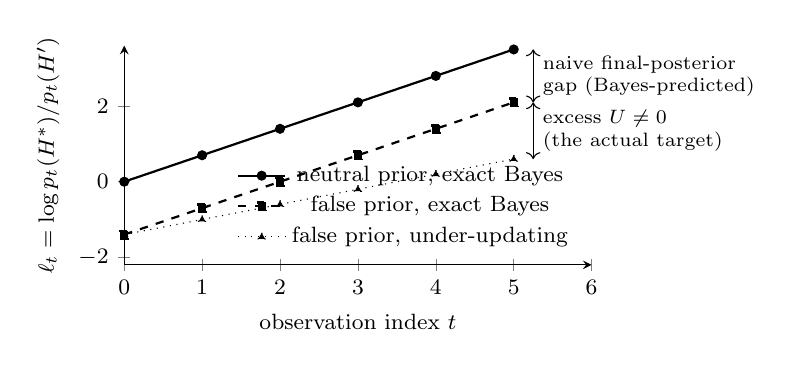
\begin{tikzpicture}
\begin{axis}[
  width=0.62\textwidth, height=0.36\textwidth,
  xlabel={observation index $t$},
  ylabel={$\ell_t = \log p_t(H^*)/p_t(H')$},
  xmin=0, xmax=6, ymin=-2.2, ymax=3.6,
  xtick={0,1,...,6},
  legend style={at={(0.98,0.03)},anchor=south east,font=\footnotesize,draw=none,fill=none},
  axis lines=left, tick label style={font=\footnotesize}, label style={font=\footnotesize},
  clip=false,
]
\addplot[black, thick, mark=*, mark size=1.4pt] coordinates {(0,0) (1,0.7) (2,1.4) (3,2.1) (4,2.8) (5,3.5)};
\addlegendentry{neutral prior, exact Bayes}
\addplot[black, thick, dashed, mark=square*, mark size=1.4pt] coordinates {(0,-1.4) (1,-0.7) (2,0) (3,0.7) (4,1.4) (5,2.1)};
\addlegendentry{false prior, exact Bayes}
\addplot[black, thin, dotted, mark=triangle*, mark size=1.4pt] coordinates {(0,-1.4) (1,-1.0) (2,-0.6) (3,-0.2) (4,0.2) (5,0.6)};
\addlegendentry{false prior, under-updating}
% annotations
\draw[<->,thin] (axis cs:5.25,2.1) -- (axis cs:5.25,3.5) node[midway,right,font=\scriptsize,align=left] {naive final-posterior\\gap (Bayes-predicted)};
\draw[<->,thin] (axis cs:5.25,0.6) -- (axis cs:5.25,2.1) node[midway,right,font=\scriptsize,align=left] {excess $U\neq 0$\\(the actual target)};
\end{axis}
\end{tikzpicture}
\caption{Schematic, not data. Two exact Bayesians shown the same evidence move by the same $\Delta\ell$ and end at different posteriors; the final-posterior gap is fully predicted by the prior gap. Only a difference in \emph{movement} (dotted line) is evidence about evidence processing. Our early ``confirmation bias'' result was the upper gap. Illustrative slopes of $0.7$ and $0.4$ nats per observation.}
\label{fig:logodds}
\end{figure}

% ===========================================================================
\section{Same-Prior Normative Framework}
\label{sec:framework}

The same-prior idea is simple to state and easy to get wrong. Four things have to be pinned down: the world, what the model knows, which belief the oracle uses, and how the prior is induced. Figure~\ref{fig:pipeline} shows how the pieces fit.

\begin{figure}[t]
\centering
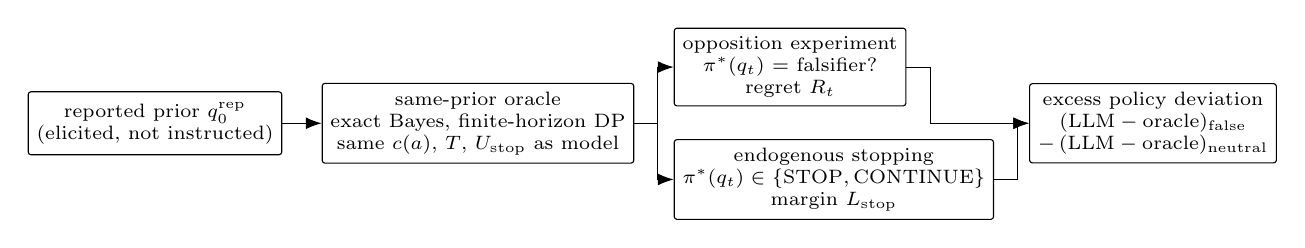
\begin{tikzpicture}[
  node distance=4mm and 5mm,
  box/.style={draw, rectangle, rounded corners=1pt, align=center, font=\scriptsize, inner sep=3pt, minimum height=8mm},
  arr/.style={-{Latex[length=2mm]}, thin},
]
\node[box] (prior) {reported prior $q_0^{\rep}$\\(elicited, not instructed)};
\node[box, right=of prior] (oracle) {same-prior oracle\\exact Bayes, finite-horizon DP\\same $c(a)$, $T$, $\Ustop$ as model};
\node[box, above right=2mm and 5mm of oracle, anchor=west] (opp) {opposition experiment\\$\pi^*(q_t)$ = falsifier?\\regret $R_t$};
\node[box, below right=2mm and 5mm of oracle, anchor=west] (stop) {endogenous stopping\\$\pi^*(q_t)\in\{\STOP,\CONT\}$\\margin $\Lstop$};
\node[box, right=of $(opp.east)!0.5!(stop.east)$, xshift=5mm] (dev) {excess policy deviation\\$(\text{LLM}-\text{oracle})_{\text{false}}$\\$-\,(\text{LLM}-\text{oracle})_{\text{neutral}}$};
\draw[arr] (prior) -- (oracle);
\draw[arr] (oracle.east) -- ++(3mm,0) |- (opp.west);
\draw[arr] (oracle.east) -- ++(3mm,0) |- (stop.west);
\draw[arr] (opp.east) -- ++(3mm,0) |- (dev.west);
\draw[arr] (stop.east) -- ++(3mm,0) |- (dev.west);
\end{tikzpicture}
\caption{The comparison. The oracle is initialized with the model's own reported belief and solves the model's own decision problem. The estimand is never ``LLM vs.\ oracle'' alone but the false-minus-neutral difference of that gap, so that generic incompetence at the task cancels.}
\label{fig:pipeline}
\end{figure}

\subsection{The world}
\label{sec:world}

A world has a finite hypothesis set $\Hset = \{h_1,\dots,h_n\}$, a finite experiment menu $\Aset = \{a_1,\dots,a_m\}$, a finite outcome space $\Yset$, and known outcome likelihoods $P(y\mid h,a)$ for every combination. One hypothesis $h^* \in \Hset$ is true. In the false-prior condition the model is induced to favor a specific false hypothesis $H' \neq h^*$. Given a belief $q_t$ over $\Hset$ and an observed outcome $y_t$ from experiment $a_t$, the exact update is ordinary Bayes:
\begin{equation}
q_{t+1}(h) \;=\; \Bop(q_t; a_t, y_t)(h) \;=\; \frac{q_t(h)\,P(y_t\mid h,a_t)}{\sum_{j} q_t(h_j)\,P(y_t\mid h_j,a_t)}.
\label{eq:bayes}
\end{equation}
Because everything is known, the oracle can compute the value of any experiment and of stopping. It knows nothing about the truth that the model does not.

\subsection{What the model knows}
\label{sec:knows}

The model and the oracle must face the same information problem. In the primary synthetic studies the model is given the hypothesis set, the experiment menu, the outcome space, the likelihood structure, the remaining horizon, experiment costs, and the terminal objective. This makes the task partly computational. That is intentional. We first check that the model can do the computation in a neutral condition (Section~\ref{sec:competence}), and only then ask whether a false prior makes it deviate.

\subsection{The oracle's decision problem}
\label{sec:dp}

Both primary studies use one decision problem, so we define it once. At a decision with remaining horizon $\tau$ and belief $q$, the agent either stops or runs an experiment $a$ at cost $c(a)$. Stopping yields terminal utility $\Ustop(q)$. Write $P_q(y\mid a) = \sum_h q(h) P(y\mid h,a)$ for the agent's predictive distribution. Then
\begin{align}
V_\tau(q) &= \max\Big[\, \Ustop(q),\; \max_{a\in\Aset} Q_\tau(q,a) \Big], \qquad V_0(q) = \Ustop(q), \label{eq:V}\\
Q_\tau(q,a) &= -c(a) + \sum_{y\in\Yset} P_q(y\mid a)\, V_{\tau-1}\big(\Bop(q;a,y)\big). \label{eq:Q}
\end{align}
The oracle policy $\pi^*_\tau(q)$ is the maximizer over $\Aset \cup \{\STOP\}$.

The terminal utility is a strictly proper scoring rule $S(r,h)$ \citep{gneiting2007strictly} applied to a reported final belief $r$ when the truth is $h$. From the agent's own point of view, $\Ustop(q) = \max_r \sum_h q(h)\,S(r,h) = \sum_h q(h)\,S(q,h)$, because properness makes honest reporting optimal. Under the log score this is $-\mathrm{H}(q)$ up to a constant, and the one-step continuation value becomes
\begin{equation}
Q_1(q,a) - \Ustop(q) \;=\; \mathrm{EIG}(a;q) - c(a),
\label{eq:eig}
\end{equation}
the expected information gain of the experiment net of its cost. This is why the two primary studies are the same objective viewed from two decisions: which experiment, and whether any experiment.

\paragraph{Cost, horizon, and objective are shared.}
The model receives exactly the cost function $c$, horizon $T$, and scoring rule $S$ that the oracle optimizes, stated in the prompt. We never tell the model ``stop when you are confident'' while the oracle optimizes something else. If we did that, we would have built the artifact ourselves.

\subsection{Which belief the oracle uses}
\label{sec:beliefs}

This is central, not a side analysis. A reported belief can differ from the belief a model acts on. If it says $P(H') = 0.6$ but stops as if $P(H') = 0.95$, then ``premature closure'' might just be misreporting. We therefore keep three belief objects distinct and never substitute one for another silently:
\begin{itemize}
\item $q_t^{\rep}$: the distribution the model reports when asked at decision $t$.
\item $q_t^{\Bayes} = \Bop(\cdots\Bop(q_0^{\rep}; a_0,y_0)\cdots; a_{t-1},y_{t-1})$: the model's elicited prior propagated by exact Bayes through the evidence the model actually observed.
\item $q_t^{\rev}$: a behaviorally inferred belief, defined below and used only in exploratory analysis.
\end{itemize}
For an exact Bayesian these coincide. For an LLM none of them is guaranteed to equal another, and each estimand below states which one it conditions on.

We run two oracles. The \emph{reported-belief oracle} re-elicits $q_t^{\rep}$ at each decision and asks whether the action was rational given what the model currently says: it compares $a_t^{\mathrm{LLM}}$ with $\pi^*(q_t^{\rep})$. The \emph{trajectory oracle} compares $a_t^{\mathrm{LLM}}$ with $\pi^*(q_t^{\Bayes})$ and asks whether the model's whole belief-and-action path departs from the rational one. These answer different questions. A deviation under the trajectory oracle can come from a belief-updating error, an action error, or both; a deviation under the reported-belief oracle is an action error conditional on the stated belief. We report both and do not net them against each other.

We also check that elicitation is stable across semantically equivalent probability questions \citep{sclar2024quantifying}, and record the dispersion. As an exploratory analysis we fit a one-parameter revealed belief: a scalar shift $\delta$ on the log odds of $H'$,
\begin{equation*}
q^{\rev}_t(\delta)(H') \propto q_t^{\rep}(H')\,e^{\delta}, \qquad q^{\rev}_t(\delta)(h) \propto q_t^{\rep}(h) \;\; (h\neq H'),
\end{equation*}
with $\hat\delta$ chosen per episode so that the oracle policy under $q_t^{\rev}(\hat\delta)$ best matches the model's observed decisions. If the main effect disappears under the revealed belief, the interpretation changes and we say so.

\subsection{Prior induction}
\label{sec:induction}

Telling a model $P(H') = 0.8$ does not make it believe that; instructed priors are often ignored \citep{gupta2025coinflips}. We use the elicited prior $q_0^{\rep}$, not the instructed one, and we report the gap between them. Any effect that survives the primary studies is then re-tested with a misleading-pilot induction (Section~\ref{sec:pilot}), where the model gets its false belief from honest but unlucky data instead of an instruction.

% ===========================================================================
\section{Opposition-World Experiment}
\label{sec:opposition}

If an agent strongly favors $H'$, not running the experiment most likely to kill $H'$ can be perfectly rational; positive testing is often a good strategy \citep{klayman1987confirmation}. So ``false-prior models ran fewer falsifiers'' proves nothing.

\paragraph{Falsifiers, relative to a belief.}
Whether an experiment threatens $H'$ depends on what the agent believes. Under belief $q$, define the falsification probability of $a$ as the agent's own probability that the outcome pushes $H'$ below a threshold $\theta$:
\begin{equation}
F(a;q) \;=\; \sum_{y} P_q(y\mid a)\; \Ind\!\big[\Bop(q;a,y)(H') \le \theta\big].
\label{eq:F}
\end{equation}

\paragraph{Opposition and rational-avoidance worlds.}
We search offline for \emph{opposition worlds}: the induced prior strongly favors $H'$ ($q_0(H') \ge \pi_{\min}$), $H'$ is false, and under that exact prior the rationally best experiment $a^* = \argmax_a Q_T(q_0,a)$ is still one with substantial falsification probability and a value margin over the best non-falsifier,
\begin{equation}
F(a^*;q_0) \ge \phi_{\min}, \qquad Q_T(q_0,a^*) - \max_{a:\,F(a;q_0)<\phi_{\min}} Q_T(q_0,a) \ge g_{\min}.
\label{eq:opp}
\end{equation}
In these worlds, false prior plus rational policy means run the falsifier. If the model avoids it, its own prior cannot excuse that.

We pair these with \emph{rational-avoidance worlds}, where under the same prior the oracle genuinely prefers a non-falsifying experiment ($F(a^*;q_0) < \phi_{\min}$, with the mirror-image margin). The interesting result is not that models dislike falsifiers. It is that they avoid falsifiers specifically when their own beliefs say they should not. That is an interaction between prior condition and world type, and it is what separates prior-specific avoidance from a generic habit. World type is defined relative to the false prior. Every world is also run under the neutral prior, and each condition's outcome is computed against that condition's own oracle. The thresholds $\pi_{\min}$, $\theta$, $\phi_{\min}$, $g_{\min}$ are set from oracle simulations before any model run (Section~\ref{sec:gates}).

\paragraph{Primary outcome: value regret.}
The primary outcome is the value lost by the model's choice, computed under the model's belief:
\begin{equation}
R_t \;=\; Q_\tau\big(q_t, \pi^*(q_t)\big) - Q_\tau\big(q_t, a_t^{\mathrm{LLM}}\big), \qquad q_t \in \{q_t^{\rep}, q_t^{\Bayes}\}.
\label{eq:regret}
\end{equation}
Binary ``picked the falsifier'' is secondary. Regret is the direct fix for preliminary study~3, where a model could pick the second-best action at almost no cost and still get labelled wrong. Regret is in units of the shared utility, so it is comparable across conditions, but the range of attainable regret depends on the belief state; we also report regret normalized by the oracle's best-minus-worst gap in that state as a sensitivity analysis. In this study the model must choose an experiment; $\STOP$ is not in the action set, and the primary decision is the constructed opposition state at $t=0$, with later visited states classified by the same criterion as a secondary analysis.

\paragraph{Estimand.}
Since the oracle has zero regret against itself, the prior-specific estimand in world type $w \in \{\text{opp}, \text{RA}\}$ is
\begin{equation}
\Delta^{w}_{\mathrm{opp}} \;=\; \E[R \mid \text{false}, w] - \E[R \mid \text{neutral}, w],
\label{eq:dopp}
\end{equation}
and the primary test is the interaction $\Delta^{\text{opp}}_{\mathrm{opp}} - \Delta^{\text{RA}}_{\mathrm{opp}}$. A model that is simply bad at the task has positive regret in both conditions and both world types, and drops out of this contrast.

% ===========================================================================
\section{Endogenous Stopping Experiment}
\label{sec:stopping}

This is the study with the most upside.

Most agent benchmarks force the model to keep acting. A real scientist decides when to stop. So the action set is $\Aset \cup \{\STOP\}$, and the oracle solves the finite-horizon problem of Equations~\eqref{eq:V}--\eqref{eq:Q}, an ordinary Bayesian sequential decision problem \citep{wald1947sequential,degroot1970optimal}. The oracle tells us whether another experiment is worth its cost. The event we care about is the model choosing $\STOP$ in a state where the same-prior oracle says $\CONT$. We call that \emph{premature epistemic closure}.

\paragraph{The estimand is a difference-in-differences.}
LLMs may be bad at optimal stopping in general. So the raw rate of stopping-when-oracle-continues is not the result. Let
\begin{equation}
C_k \;=\; P\big(a_t^{\mathrm{LLM}} = \STOP \;\big|\; \pi^*(q_t) \ne \STOP,\; \text{condition } k\big), \qquad k \in \{\text{false},\text{neutral}\},
\label{eq:C}
\end{equation}
where $q_t$ is again $q_t^{\rep}$ (primary) or $q_t^{\Bayes}$. The prior-specific effect is
\begin{equation}
\Delta_{\mathrm{closure}} \;=\; C_{\text{false}} - C_{\text{neutral}}.
\label{eq:dclosure}
\end{equation}
This is a generic-versus-prior-specific distinction: $C_{\text{neutral}}$ measures how badly the model stops when nothing is at stake for a favored theory, and $\Delta_{\mathrm{closure}}$ measures how much worse it gets when something is. We also report the reverse error, continuing where the oracle stops, in both conditions. A model that never stops has $C_k = 0$ and is not thereby rational; the reverse error keeps that visible.

\paragraph{State matching.}
One more thing has to be handled. The $\CONT$ states under a false prior and under a neutral prior are different sets of belief states, and they can sit at different distances from the stopping boundary. Comparing them raw can produce a spurious effect. We therefore define the stopping margin
\begin{equation}
\Lstop(q) \;=\; \max_{a} Q_\tau(q,a) - \Ustop(q),
\label{eq:Lstop}
\end{equation}
the value destroyed by stopping in that state, and include it as a covariate in the primary model. We also restrict the headline estimate to states with $\Lstop \ge \lambda$ for a prespecified $\lambda$, where each condition's margin is computed under its own belief and $\lambda$ is chosen from oracle simulations so that both conditions have adequate support. This does double duty: it fixes the state-matching problem and it separates a scientifically meaningful closure effect from one that only appears where continuing barely matters. We report $\Delta_{\mathrm{closure}}(\lambda)$ across a grid of $\lambda$ as a sensitivity analysis, and the value-weighted version $\E[\Lstop(q_t)\,\Ind[a_t^{\mathrm{LLM}}=\STOP] \mid \pi^*(q_t)\neq\STOP, k]$, which is the expected value destroyed by closure in each condition.

\paragraph{Cost and utility are not hidden.}
The stopping boundary depends on $c(a)$ and $\Ustop$. We fix one primary regime $(c, S, T)$ in advance, give it to the model, and then rerun across a prespecified range of costs and scoring-rule parameters. A real closure effect should not live at one hand-picked threshold.

% ===========================================================================
\section{Experimental Design and Validation}
\label{sec:validation}

The biggest lesson from the preliminary studies is that we kept finding out the environment was wrong after the expensive runs. The new pipeline is
\begin{equation*}
\text{mechanism} \to \text{oracle} \to \text{diagnostic regime} \to \text{synthetic validation} \to \text{freeze} \to \text{frontier models},
\end{equation*}
and no frontier-model call happens before the first four steps pass.

\subsection{Gate 1: oracle-only validation}
\label{sec:gate1}

Before any LLM call we generate worlds, compute exact updates, find opposition states and $\STOP/\CONT$ regions, and run the whole analysis on agents we control:
\begin{itemize}
\item an exact Bayesian agent, the normative baseline;
\item a \emph{falsifier-averse} agent that acts on $\tilde Q(q,a) = Q_\tau(q,a) - \kappa\,F(a;q)$ for a known $\kappa > 0$;
\item a \emph{premature-closure} agent that, for a known $\beta > 0$, acts on $\tilde U_{\mathrm{stop}}(q) = \Ustop(q) + \beta\,\Ind[\argmax_h q(h) = H']$: a bonus to $\STOP$ when its favored hypothesis is ahead.
\end{itemize}
If we implant a 10 percentage-point closure effect, the pipeline should recover roughly 10 points with useful precision. If it cannot, the benchmark is not ready and we fix it before spending anything on models. This is also what makes a later null mean something.

\subsection{World quality gates}
\label{sec:gates}

Random worlds are not automatically useful worlds. A world enters model evaluation only if it satisfies numerical constraints fixed in advance: moderate per-experiment evidence (a cap on likelihood ratios), a meaningful gap between best and second-best action value, a recoverable truth within the horizon, both real $\CONT$ and real $\STOP$ states, opposition states under the false prior with matching neutral-prior controls, and no single experiment that dominates everywhere. Thresholds come from oracle simulations, not from model behavior. We log the rejection rate; if almost every random world fails, we redesign the generator rather than lean on extreme post-selection.

\subsection{Freeze}
\label{sec:freeze}

World-selection rules, quality thresholds, metrics, and analysis code are committed to the repository before any target-model run. Selection may depend on oracle geometry. It may not depend on whether a particular model behaved interestingly. The confirmatory configuration is committed before the confirmatory run.

\subsection{Neutral competence gate}
\label{sec:competence}

We do not measure subtle prior-specific bias on a task the model fundamentally cannot solve. Before any false-prior cell, the model is run in the neutral condition. The working target is roughly 85 to 90\% oracle-optimal action choice in the relevant states, with low value regret. The number is not sacred; the principle is.

If competence is poor, we are allowed to fix task complexity, prompt, interface, or world difficulty. To keep this from becoming a degrees-of-freedom leak, we allow at most $k$ revision rounds (\todo{fix $k$}), all logged, and each revision is itself re-checked with the synthetic agents of Section~\ref{sec:gate1}. If competence is still poor after that, the model is recorded as not competent on this task and it is excluded from strong claims rather than tuned further.

% ===========================================================================
\section{Robustness and Statistical Analysis}
\label{sec:robustness}

\subsection{Prompts}
At the pilot stage, not after the paper is written, we run about five semantically equivalent prompt formulations with identical information, cost, and objective. An effect that vanishes under rewording is not a mechanism, and we want to learn that cheaply.

\subsection{Models}
Final evaluation should cover several model families. Work so far has used OpenAI GPT-5.6 Sol, xAI Grok, DeepSeek, and Google Gemma 3 12B (\todo{exact deployment strings from the logs}). The early signal that matters is not identical effect size. It is whether the direction of prior-specific deviation is the same across families.

\subsection{Dose response}
For any serious positive we vary prior strength, for example instructed $q_0(H') \in \{0.5, 0.7, 0.9\}$, analyze against the elicited prior in each cell, and ask whether excess deviation from the corresponding same-prior oracle increases monotonically. A curve is much stronger evidence than a single treatment-control gap.

\subsection{Misleading-pilot induction}
\label{sec:pilot}
The obvious objection to instructed priors is that the model is just following instructions. So any surviving effect is re-tested with priors the model earned honestly. Pilot data are drawn from the true hypothesis, $D_{\text{pilot}} \sim P(\cdot \mid h^*, a_{\text{pilot}})$, and we select finite samples for which a neutral-prior Bayesian posterior legitimately favors $H'$. The model is shown the pilot, its post-pilot belief is elicited, and that elicited belief initializes the same-prior oracle. The model becomes wrong for good reasons. If the effect reproduces, instruction-following is no longer a plausible explanation.

\subsection{Statistics and power}
\label{sec:stats}
We care about effect sizes and intervals, not isolated p-values.

For stopping, the primary model is a hierarchical logistic regression of the $\STOP$ indicator on prior condition, oracle recommendation, their interaction, $\Lstop$, and random effects for model, world, and prompt variant; the coefficient of interest is the interaction, with marginal effects reported on the probability scale. For regret and value loss we use hierarchical continuous models or bootstrap intervals across worlds.

Before any model run we simulate the full analysis with the synthetic agents and pick the per-cell $N$ that detects the smallest effect we would care about. The provisional target is 10 percentage points of excess closure in states with $\Lstop$ above threshold. The provisional design is 300 episodes per model per principal condition, to be revised by the power simulation and the API budget. The full matrix (models $\times$ worlds $\times$ conditions $\times$ prompt variants $\times$ replicates) is written down before final runs. If it is too expensive, we cut prompt variants and replicates before we cut model families.

% ===========================================================================
\section{Conditional Allocation Extension}
\label{sec:allocation}

Only if the decision rules of Section~\ref{sec:plan} send us here. The scientist has several open projects $X_1,\dots,X_k$ and one budget, and at each step chooses which project gets the next experiment. For two projects let $M = V_X - V_Y$ be the difference in rational marginal value. A rational agent should switch near $M = 0$. If false-prior agents require substantially larger $M$ before returning to the question that threatens their belief, that is an implicit shadow cost on disconfirmatory inquiry. Deferred until earned.

Pruning, theory-family lock-in, prior provenance, self-generated theory ownership, revision thresholds, and downstream propagation are directions for later work. They are not commitments in this proposal.

% ===========================================================================
\section{Related Work}
\label{sec:related}

Our central comparison is an LLM's scientific policy against an exact Bayesian policy that starts from the LLM's own reported belief. Several literatures touch one piece of this. None that we found combines a planted false prior, a same-belief normative policy, and an outcome defined on experiment choice and stopping. We go through them and say where the closest neighbors differ.

\paragraph{Bayesian experimental design and LLM information gathering.}
The normative machinery is classical: \citet{lindley1956measure} defines the expected information of an experiment, \citet{chaloner1995bayesian} put design choice inside expected-utility maximization, which is what makes ``optimal'' depend on the utility, \citet{rainforth2024modern} and \citet{foster2021deep} cover the modern sequential versions, and \citet{cheng2025optimal} treat the coupled design-and-stopping problem without LLMs. The closest methodological neighbor is BED-LLM \citep{choudhury2026bedllm}, which builds a probabilistic model from LLM-sampled hypotheses and LLM likelihoods, chooses each query by expected information gain, and filters hypotheses incompatible with the history. Its motivation already notes that LLM priors are ``heavily overconfident on a small number of possible hypotheses'' and that models ``exhibit premature overconfidence.'' The difference from our work is what the Bayesian policy is for. BED-LLM uses it as a method to make the LLM a better asker and evaluates task success against prompting baselines, with fixed query budgets and no cost-aware stopping. We use an exact same-belief policy as a control, inject false priors as a treatment, and measure regret and stop/continue disagreement against it. Related methods use information-gain planning \citep{hu2024uncertainty}, probabilistic programs over LLM-proposed rules \citep{piriyakulkij2024doing}, or EIG as a training signal \citep{mazzaccara2024learning}. \citet{grand2026shoot} is the one LLM paper we found with an explicit ask-versus-act rule and an EIG-optimal reference, but the reference is computed under the ground-truth posterior, so it cannot separate false belief from policy distortion. On the evaluation side, BoxingGym \citep{gandhi2025boxinggym} scores LLM designs by information regret against the environment's true model, and \citet{ke2024foundation} compare against an information-gain optimum that assumes perfect reasoning. Neither conditions on what the model believes.

\paragraph{Autonomous AI scientists and their benchmarks.}
End-to-end systems now generate ideas, run experiments, and write papers \citep{lu2024aiscientist,yamada2025aiscientistv2}, drive laboratory hardware \citep{boiko2023coscientist}, rank hypotheses at scale \citep{gottweis2026coscientist}, and produce wet-lab-validated designs \citep{swanson2025virtuallab}. They are evaluated on output quality or task success, which leaves the inquiry policy unexamined: AI Scientist-v2's tree search over experiments is a research policy, and it is scored only through the resulting paper. \citet{riosgarcia2026aiscientists} find, across many agent traces, that evidence is frequently ignored and refutation-driven revision is rare, and \citet{bisht2026notbuilt} argue that single-turn benchmarks without experimental feedback cannot see this. AutoDiscovery \citep{agarwal2025autodiscovery,agarwal2026evidence} elicits the LLM's own prior and posterior over hypotheses but uses their difference as a search reward, not as a standard for judging the agent; \citet{shah2026whenstop} ask when an AI scientist should stop, with classical model discrimination and no LLM decision-maker. Static benchmarks score answers, code, or plans \citep{wang2026frontierscience,liu2026lifescibench,xu2025sgibench,chen2025scienceagentbench,majumder2025discoverybench,liu2026scope}; SCOPE's ``experimental design'' means planning the experiments of an ML paper. Interactive benchmarks exercise closed-loop experiment selection but score final task success \citep{jansen2024discoveryworld,wiemann2026discoverphysics,chen2025physgym,malik2026made,kabra2026autoscilab}; PhysGym varies the prior knowledge \emph{given} to the agent, not the prior the agent holds. Hybrid systems put an LLM inside Bayesian optimization \citep{liu2024llambo,kristiadi2024sober,rankovic2026uncertainty} or next to a value-of-information selector \citep{murphy2026mda,cisse2026closedloop}, imposing a Bayesian selector rather than testing whether the LLM's own selections are Bayesian-consistent. \citet{gupta2025llmsbo} report that LLM agents used directly as optimizers show no sensitivity to experimental feedback: permuting outcome labels does not change performance. That is a policy-level failure of the kind we want to measure, but measured without a belief state.

\paragraph{Belief elicitation and stated versus revealed beliefs.}
Our oracle is initialized from a verbalized probability distribution, so it inherits what is known about verbalized calibration \citep{kadavath2022language,lin2022teaching,tian2023just,xiong2024can}, including overconfidence and dependence on how the question is asked, which is why we test elicitation across paraphrases \citep{sclar2024quantifying,mizrahi2024state,xia2026calibration}. The stronger concern, that the belief a model states is not the belief it acts on, has its own recent literature. \citet{yamin2026when} jointly elicit probabilities and decisions in threshold-decision tasks and derive utility-free conditions for the stated belief to rationalize the decision; a companion paper fits revealed utilities given elicited beliefs \citep{yamin2026revealed}. \citet{pal2025knowing} find models betting against their own high-confidence answers and failing to seek information when confidence is low; \citet{wang2026faithful} find verbal confidence that does not respond to error costs as an expected-utility maximizer's would; \citet{sobotka2026why} locate the weak link in belief-to-action conversion; \citet{mondal2026implicit} contrast explicit answers with token-level probabilities; \citet{kumaran2026causal} show, in the other direction, that verbal confidence does partly drive abstention. Stated probabilities can also be internally incoherent \citep{zhu2024incoherent}. Our two-oracle design and the revealed-belief fit $\hat\delta$ (Section~\ref{sec:beliefs}) are our engagement with this measurement problem. What is new here is applying the belief-versus-action test to sequential experiment choice and stopping rather than to one-shot decisions.

\paragraph{LLMs as Bayesian updaters.}
Whether in-context updating is Bayesian is contested \citep{xie2022explanation,falck2024icl}. \citet{gupta2025coinflips} find that instructed priors are often ignored while subsequent updates track Bayes, the direct precedent for our instructed-versus-elicited prior check. \citet{chen2026notbayesian} elicit an LLM's own prior and likelihood and compare its stated posterior with the exact Bayes posterior computed from those same quantities. That is the same-belief-control idea applied to passive updating, and the closest existing use of an LLM's own beliefs as the seed of an exact Bayesian computation. Our extension is from inference to policy: which experiment, and whether to run one at all. BayesBench \citep{samanta2026bayesbench}, the martingale score \citep{he2025martingale}, \citet{schubert2024asymmetric}, and \citet{qiu2025bayesian} likewise diagnose belief trajectories with evidence supplied exogenously.

\paragraph{Sycophancy, consistency, and commitment.}
Sycophancy is agreement with a user's stated view \citep{perez2023discovering,sharma2024towards,wei2023simple}. Belief persistence under contradictory documents \citep{xie2024adaptive,wan2024evidence}, capitulation under challenge \citep{wang2023defend,xie2024askagain,huang2024cannot}, and confidence escalation in debate \citep{prasad2025debate} are related phenomena. \citet{atwell2025basil} score sycophantic belief shifts as deviations from Bayesian consistency, the nearest of these to our framing, but the outcome is a belief and the perturbation is user input. \citet{batista2026rational} give a rational analysis in which a Bayesian fed data conditioned on its own hypothesis grows confident without approaching the truth; the agents there are humans, but the mechanism is the one we test in the LLM's own policy. In all of these the outcome is agreement or textual persistence. Ours is a scientific action relative to a same-prior normative policy, with no user opinion in play.

\paragraph{Confirmation bias and classical foundations.}
Cognitive-bias batteries \citep{binz2023cognitive,echterhoff2024cognitive,macmillanscott2024irrationality} find LLM errors that are often not human-like and are unstable across repeats. Closest to our opposition experiment, \citet{jhaveri2026failing} port Wason's 2-4-6 task \citep{wason1960failure} to LLMs and measure confirmation bias as the ratio of hypothesis-incompatible to hypothesis-compatible tests relative to the model's own stated hypothesis; FalsifyBench \citep{bertolazzi2026falsifybench} does likewise with semantic rules. Both observe the phenomenon we care about, with no manipulated prior and no Bayesian reference policy, so a preference for compatible tests cannot be told apart from a rational positive test strategy. That distinction is old: \citet{klayman1987confirmation} showed positive testing is often a good heuristic, and \citet{oaksford1994rational} showed selection-task choices look rational as optimal data selection. Both are the reason our outcome is value regret against an environment-specific oracle rather than a count of falsifiers. \citet{nickerson1998confirmation} separates search-level from interpretation-level bias, which is the split between our fixed-evidence preliminary studies and the two primary experiments; \citet{lord1979biased} and \citet{kunda1990case} are the interpretation-side precedents. For stopping and value of information we rely on \citet{wald1947sequential}, \citet{raiffa1961applied}, \citet{howard1966information}, and \citet{degroot1970optimal}.

\paragraph{Positioning.}
Existing scientific-agent evaluations primarily assess task performance, experiment quality, or information gathering. We instead ask whether an agent's scientific policy is rational conditional on its own belief state, which lets false belief be separated from policy distortion. The ingredients exist separately: exact Bayes seeded with the model's own beliefs for passive updating \citep{chen2026notbayesian}, belief-versus-action consistency for one-shot decisions \citep{yamin2026when}, EIG policies built from LLM beliefs as a method \citep{choudhury2026bedllm}, and belief-threatening test avoidance measured heuristically \citep{jhaveri2026failing}. We did not find work that puts them together for sequential experiment choice and endogenous stopping under a controlled false prior. We make no stronger novelty claim than that.

% ===========================================================================
\section{Limitations and Failure Modes}
\label{sec:limitations}

Each item names the way the result could be wrong and the control already in the design.

\begin{enumerate}
\item \textbf{Stated beliefs may not equal decision-relevant beliefs.} The oracle is only as good as $q_t^{\rep}$. Controls: two oracles (reported-belief and trajectory), elicitation-stability checks across paraphrases, and the exploratory revealed-belief fit $\hat\delta$ (Section~\ref{sec:beliefs}). If the effect survives only under the stated belief, we report that as the finding.
\item \textbf{Utility and cost assumptions determine the stopping oracle.} There is no prior-free ``right time to stop.'' Controls: one primary regime fixed and disclosed to the model in advance; a prespecified sweep over cost and scoring-rule parameters (Section~\ref{sec:stopping}).
\item \textbf{Synthetic worlds may not generalize to real science.} Finite hypothesis sets with known likelihoods are a cartoon of research. Controls: the design trades realism for an exact oracle on purpose, after preliminary study~4 showed that real data without an oracle cannot answer the question; generalization is a claim for later work, not this one.
\item \textbf{Generic task incompetence can mimic bias.} Controls: the neutral competence gate (Section~\ref{sec:competence}); all estimands are false-minus-neutral differences against each condition's own oracle; the reverse stopping error is reported alongside closure.
\item \textbf{Prompt sensitivity.} Controls: about five equivalent formulations at the pilot stage, with prompt variant as a random effect (Section~\ref{sec:robustness}).
\item \textbf{Model-family heterogeneity.} Controls: several families, with the sign of the prior-specific deviation as the cross-family criterion, not effect size; models failing the competence gate are excluded from strong claims rather than tuned.
\item \textbf{World engineering creates researcher degrees of freedom.} Opposition worlds are searched for, and search can find anything. Controls: selection rules depend only on oracle geometry; thresholds are set from oracle simulations; the configuration is frozen before confirmatory runs and the world rejection rate is logged (Sections~\ref{sec:gates}--\ref{sec:freeze}).
\item \textbf{Selective mechanism search after nulls.} Two primary mechanisms and one conditional extension are already several chances to find something. Control: the falsification rule in Section~\ref{sec:plan}, which specifies in advance when we stop.
\end{enumerate}

% ===========================================================================
\section{Research Plan and Decision Rules}
\label{sec:plan}

\subsection{What would falsify our story}

Our preferred story is weakened if false-prior models track same-prior optimal choice in opposition worlds, show little prior-specific excess closure, and those nulls hold across models and prompts, while the synthetic agents show the benchmark would have caught an effect of meaningful size at the power we ran.

If that happens, we do not invent another confirmation-bias metric. The result becomes: much of the apparent confirmation bias in AI scientific agents disappears once the rational consequences of different priors are controlled. That is a real paper, provided the benchmark is demonstrably sensitive.

\medskip
\noindent\emph{Falsification rule.} If opposition and stopping are both null, neutral competence is high, the synthetic biased agents are detectable, and the uncertainty intervals exclude effects of the prespecified meaningful size, we stop mechanism hunting and write the robustness and null result.
\medskip

Two outcomes are useful. Either local inference is robust and false priors distort inquiry policy, in which case the conclusion is roughly that false priors do not make AI scientists reject evidence so much as make unresolved questions look finished. Or models track their same-prior controls everywhere, in which case some apparent confirmation-bias effects may reflect rational consequences of different priors. Both answer the same question.

\subsection{Decision rules}
\begin{itemize}
\item \textbf{Opposition positive.} Do not add a mechanism. Replicate on held-out worlds, run the prompt sweep, add model families, run the dose-response, reproduce with misleading-pilot induction.
\item \textbf{Stopping positive.} It becomes the flagship. Quantify closure rate, value destroyed, belief-state robustness, and cost/utility sensitivity.
\item \textbf{Both robust.} Allocation (Section~\ref{sec:allocation}) becomes the consequential extension.
\item \textbf{Both null and the benchmark is sensitive.} Stop hunting. Write the robustness paper.
\end{itemize}

\subsection{Gates}

\begin{table}[h]
\centering\small
\caption{Plan. Allocation comes after gate 4, not before.}
\label{tab:plan}
\begin{tabular}{@{}l p{7.4cm} l l@{}}
\toprule
Gate & What has to be true to pass & Owner & Target \\
\midrule
1. Oracle and measurement & Exact oracle, opposition generator, stopping DP, both synthetic agents, simulated analysis recovers implanted effects & \todo{name} & \todo{week} \\
2. Opposition pilot & Neutral competence passed; opposition $\times$ rational-avoidance run on available families & \todo{name} & \todo{week} \\
3. Stopping pilot & Shared cost/utility spec; prior-specific excess closure and value loss estimated & \todo{name} & \todo{week} \\
4. Confirmation & Held-out worlds, prompt sweep, dose-response, extra families, misleading-pilot replication & \todo{name} & \todo{week} \\
\bottomrule
\end{tabular}
\end{table}

\subsection{The arc}

The arc is short. Different priors rationally imply different behavior. So compare to a rational scientist with the same prior. Under that comparison, simple evidence-assimilation bias mostly disappears. So test whether the distortion has moved to the control of inquiry itself.

The question is no longer whether an AI scientist can update when contradictory evidence arrives. It is whether it will keep doing the science that lets the contradiction arrive at all.

\bibliographystyle{plainnat}
\bibliography{references}

\end{document}
